\documentclass[12pt]{article}

% Packages
\usepackage{hyperref}
\usepackage[utf8]{inputenc}
\usepackage{graphicx}
\usepackage{color}
\usepackage{afterpage}

% Author and project setup
\author{Chelcea Claudiu-Marian}
\title{Dezvoltarea de jocuri video - ce motor grafic s\^{a} folosesc?}
\date{03.18.2021}
\renewcommand{\contentsname}{Cuprins}
\renewcommand{\refname}{Bibliografie}
\setlength{\arrayrulewidth}{1mm}
\setlength{\tabcolsep}{18pt}
\renewcommand{\arraystretch}{1.5}
\addtocontents{toc}{\protect\enlargethispage{\baselineskip}}

% Main code
\begin{document}

% Intro page
\begin{titlepage}
  \afterpage{\pagecolor{white}}%
  \LARGE
  \begin{center}
  \begin{figure}
  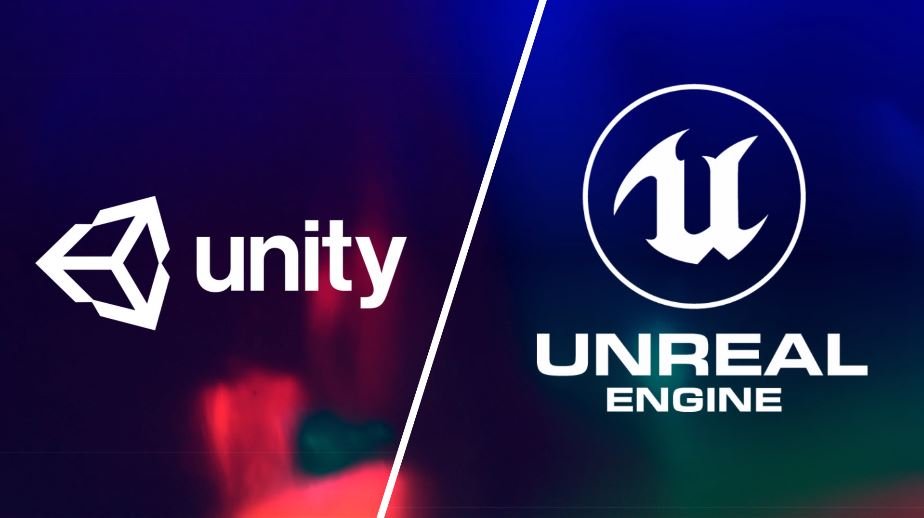
\includegraphics[width=\linewidth]{UnrealUnity.jpg}
  \caption{Unity vs Unreal Engine,  credits to \href{https://www.htlo.co.uk/unity-vs-unreal-engine-a-quick-comparison/}{HTLO}.}
  \label{fig:UvsUE}

\end{figure}

    {\bfseries Dezvoltarea de jocuri video - ce motor grafic s\^{a} folosesc?}\\[3em]
    {\large
      \begin{tabular}{rl}
      \textbf{Nume:} & Chelcea Claudiu-Marian \\
      \textbf{Grupa:} & 312CA \\
 	\textbf{Data:} & 03.19.2021
      \end{tabular}%
    }
  \end{center}
\end{titlepage}

% Contents page
\newpage
\tableofcontents

% First page
\newpage
\section{De ce un motor grafic?}
\hspace{10pt}
Un motor grafic este un sistem conceput pentru crearea și dezvoltarea de {\it jocuri video}. \par Există mai multe motoare de joc, care sunt proiectate să funcționeze pe console de jocuri video și calculatoare personale. \par Funcționalitatea de bază oferită de obicei de un motor grafic include un motor de randare (engleză renderer) pentru grafică {\bf 2D} sau {\bf 3D}, un motor de fizică sau de detectare a coliziunilor (și răspunsul la coliziune), sunet, scripting, animație, inteligență artificială, în rețea, streaming, memorie de management, suport de localizare, etc. \par Procesul de dezvoltare a jocului este de multe ori economisit, în mare parte, prin reutilizarea / adaptarea unui motor asemănător pentru a crea jocuri diferite.

% Second page
\newpage
\section{Ce motoare grafice sunt populare?}
\hspace{5pt} Lista celor mai populare 10 motoare grafice, conform \href{https://www.gamedesigning.org/career/video-game-engines/}{GAMEDESIGNING}:\footnote[1]{Aceste statistici sunt actuale la data de 19 Martie 2021.} 
\begin{itemize}
  \item Unreal Engine.
  \item Unity
  \item GameMaker
  \item Godot
  \item AppGameKit
  \item CryEngine
  \item Amazon Lumberyard
  \item RPG MAKER
  \item LIBGDX
  \item URHO3D
\end{itemize}


O analiză de la Gamasutra a constatat că Unreal și Unity sunt printre cele mai populare motoare de joc. Această analiză s-a bazat pe jocuri lansate pe Steam și Itch.io.

% Third page
\newpage
\section{Diferen\c{t}e dintre Unity si Unreal Engine}
Răspunsul la care este mai bun este o chestiune dificilă. Unii vor susține că Unreal este mai bun doar pentru faptul că este o alegere de top pentru studiourile AAA. Cu toate acestea, alții vor cita faptul că Unity este mai bine rotunjită și, pentru dezvoltatorii independenți, este adesea o intrare mai bună în industrie. Obiectiv, însă, este unul mai bun decât celălalt?

\subsection{Unity}
Unity este frecvent utilizată deoarece este:
\begin{itemize}
\item O platformă de creare 3D deschisă și avansată în timp real.
\item Folosit pentru a produce jocuri în mai multe genuri.
\item Integrat cu instrumente cheie de dezvoltare a jocurilor, inclusiv IDE-uri, instrumente grafice și controlul versiunilor.
\end{itemize}

\subsection{Unreal Engine}
Unreal Engine este frecvent utilizat deoarece este:
\begin{itemize}
\item Un motor de joc multiplataforma, cu suport pentru peste 25 de platforme.
\item O platformă de dezvoltare 3D în timp real.
\item Integrat cu instrumente cheie de dezvoltare a jocurilor, inclusiv IDE-uri, instrumente grafice și controlul versiunilor.
\end{itemize}

% Fourth page
\newpage
\section{B\u{a}t\u{a}lia final\u{a}}
\begin{tabular}{ |p{3cm}|p{3cm}|p{3cm}|  }
\hline
\multicolumn{3}{|c|}{Unreal Engine versus Unity} \\
\hline
& Unity & Unreal Engine \\
\hline
%Pret & \text{Gratuit | 125$ pe luna | 5\% din profit} & \text{Gratuit | 5\% din profit} \\
Usurinta de utilizare & Interfata simpla, mai multe surse de invatare   & Interfata grea, resurse de invatare putine \\
Utilizare & BluePrint ( clase ) - necesita programare & VisualScripting sau Coding - nu necesita programare \\
Limbaj de programare  & C-sharp &  Cplusplus \\
Grafica & Grafica este buna spre foarte buna & Cele mai bune grafici oferite de un motor grafic \\
\hline
\end{tabular}

% Bibliography
\newpage
\begin{thebibliography}{}
\bibitem{text1} 
\href{https://ro.wikipedia.org/wiki/Motor_grafic}{Wikipedia: motor grafic link}
\bibitem{text1} 
\href{https://www.gamedesigning.org/career/video-game-engines/}{Gamedesigning: website link}
\bibitem{text1} 
\href{https://www.gamasutra.com/}{Gamasutra: website link}
\bibitem{text1}
\href{https://www.htlo.co.uk/unity-vs-unreal-engine-a-quick-comparison/}{HTLO: website link}
\bibitem{text1}
\href{https://gamedevacademy.org/unity-vs-unreal/}{GameDev Academy: website link}
\end{thebibliography}

\end{document}
